% -*- coding: utf-8 -*-
% LuaLaTeX 用ドキュメント
% コンパイル: lualatex TrivialCounterexamples.tex

\documentclass[a4paper,11pt]{ltjsarticle}

% LuaTeX-ja 設定
\usepackage{luatexja}
\usepackage{luatexja-fontspec}

% 数学関連
\usepackage{amsmath,amssymb,amsthm}
\usepackage{mathtools}

% 図式・TikZ
\usepackage{tikz}
\usetikzlibrary{arrows.meta,positioning,calc,decorations.pathmorphing,shapes.geometric,patterns}
\usepackage{tikz-cd}

% ハイパーリンク
\usepackage{hyperref}
\hypersetup{
    colorlinks=true,
    linkcolor=blue!70!black,
    urlcolor=blue!50!black
}

% コード表示
\usepackage{listings}
\lstset{
    basicstyle=\ttfamily\small,
    keywordstyle=\color{blue!80!black}\bfseries,
    commentstyle=\color{green!50!black}\itshape,
    stringstyle=\color{red!70!black},
    frame=single,
    breaklines=true,
    numbers=left,
    numberstyle=\tiny\color{gray},
    xleftmargin=2em,
    framexleftmargin=1.5em,
    backgroundcolor=\color{gray!5}
}

% 色
\usepackage{xcolor}

% 定理環境
\theoremstyle{definition}
\newtheorem{definition}{定義}[section]
\newtheorem{example}[definition]{例}
\newtheorem{nonexample}[definition]{非例}
\newtheorem{counterexample}[definition]{反例}

\theoremstyle{plain}
\newtheorem{theorem}[definition]{定理}
\newtheorem{proposition}[definition]{命題}
\newtheorem{lemma}[definition]{補題}

\theoremstyle{remark}
\newtheorem{remark}[definition]{注意}

% カスタムコマンド
\newcommand{\N}{\mathbb{N}}
\newcommand{\Z}{\mathbb{Z}}
\newcommand{\Layer}{\mathrm{layer}}
\newcommand{\minLayer}{\mathrm{minLayer}}
\newcommand{\rank}{\mathrm{rank}}

% タイトル
\title{%
    \textbf{構造塔の自明例・標準例・反例}\\[0.5em]
    \Large Trivial, Canonical, and Counterexamples
}

\author{su\thanks{Lean ソースコードおよび本 \TeX 文書ともに AI ツール Antigravity (Google DeepMind) を使用して作成しました。}}

\date{2025年12月27日}

\begin{document}

\maketitle

\begin{abstract}
本文書は、構造塔（Structure Tower）理論における自明例・標準例・境界例・反例を
数学的に解説する。Lean 4 で形式化された6つの例について、定義・公理の成立/失敗・
数学的意義を示す。特に、公理の独立性と添字順序の影響を明確化する。
\end{abstract}

\tableofcontents

\newpage

%=============================================================================
\section{導入}
%=============================================================================

構造塔は以下の3つの公理によって特徴づけられる：

\begin{enumerate}
    \item \textbf{被覆性}：$\forall x \in X,\ \exists i \in I,\ x \in \Layer(i)$
    \item \textbf{単調性}：$\forall i \leq j,\ \Layer(i) \subseteq \Layer(j)$
    \item \textbf{最小性}：$\minLayer(x)$ は $x$ が属する層の最小添字
\end{enumerate}

本稿では、これらの公理がどのように成立/失敗するかを具体例で示す。

%=============================================================================
\section{自明例・標準例（Trivial.lean）}
%=============================================================================

\subsection{pointTower：単点塔}

\begin{example}[単点塔]
最も自明な構造塔。
\begin{align*}
    X &= \{*\} \quad (\text{Unit 型}) \\
    I &= \N \\
    \Layer(n) &= \{*\} \quad (\forall n \in \N) \\
    \minLayer(*) &= 0
\end{align*}
\end{example}

\begin{figure}[htbp]
\centering
\begin{tikzpicture}[
    layer/.style={draw=blue!70, fill=blue!10, minimum width=3cm, minimum height=0.6cm},
    pt/.style={circle, draw=black!70, fill=green!30, minimum size=0.5cm, font=\small}
]
\node[layer] (l0) at (0, 2) {};
\node[layer] (l1) at (0, 1) {};
\node[layer] (l2) at (0, 0) {};
\node[layer] (l3) at (0, -1) {};

\node[left=0.3cm of l0] {$\Layer(0)$};
\node[left=0.3cm of l1] {$\Layer(1)$};
\node[left=0.3cm of l2] {$\Layer(2)$};
\node[left=0.3cm of l3] {$\Layer(3)$};

\node[pt] at (0, 2) {$*$};
\node[pt] at (0, 1) {$*$};
\node[pt] at (0, 0) {$*$};
\node[pt] at (0, -1) {$*$};

\node[right=1.5cm of l0, green!50!black, font=\small] {全層が同一};

\draw[-Stealth, blue!50, thick] (l0.south) -- (l1.north);
\draw[-Stealth, blue!50, thick] (l1.south) -- (l2.north);
\draw[-Stealth, blue!50, thick] (l2.south) -- (l3.north);
\node[blue!50, font=\scriptsize] at (-2.2, 0.5) {$\subseteq$};
\end{tikzpicture}
\caption{単点塔：すべての層が $\{*\}$ で一致}
\label{fig:point-tower}
\end{figure}

\begin{theorem}
単点塔はすべての公理を満たす。
\end{theorem}

\begin{proof}
\textbf{被覆性}：$* \in \Layer(0)$ より成立。
\textbf{単調性}：$\Layer(i) = \Layer(j) = \{*\}$ なので自明。
\textbf{最小性}：$\minLayer(*) = 0$ は任意の $n$ 以下。
\end{proof}

%-----------------------------------------------------------------------------
\subsection{singletonLayerTower：単調性失敗}

\begin{nonexample}[singleton 層塔]
各層が単元集合である「塔もどき」。
\begin{align*}
    X &= \N \\
    \Layer(n) &= \{n\}
\end{align*}
\end{nonexample}

\begin{figure}[htbp]
\centering
\begin{tikzpicture}[
    layer/.style={draw=blue!70, fill=blue!10, minimum width=3cm, minimum height=0.6cm},
    elem/.style={circle, draw=black!70, fill=white, minimum size=0.5cm, font=\small}
]
\node[layer] (l0) at (0, 2) {};
\node[layer] (l1) at (0, 1) {};
\node[layer] (l2) at (0, 0) {};
\node[layer] (l3) at (0, -1) {};

\node[left=0.3cm of l0] {$\Layer(0)$};
\node[left=0.3cm of l1] {$\Layer(1)$};
\node[left=0.3cm of l2] {$\Layer(2)$};
\node[left=0.3cm of l3] {$\Layer(3)$};

\node[elem] at (0, 2) {0};
\node[elem] at (0, 1) {1};
\node[elem] at (0, 0) {2};
\node[elem] at (0, -1) {3};

% 単調性失敗を示す
\draw[red!70, thick, dashed, -Stealth] (l0.south) -- (l1.north)
    node[midway, right, font=\small, red!70] {$\not\subseteq$};

\node[text width=4cm, align=left, font=\small] at (4, 0.5) {
    $0 \leq 1$ だが\\
    $\{0\} \not\subseteq \{1\}$\\[0.3em]
    \textcolor{red!70}{\textbf{単調性失敗！}}
};
\end{tikzpicture}
\caption{singleton 層塔：単調性が壊れる}
\label{fig:singleton-tower}
\end{figure}

\begin{theorem}
singleton 層塔は被覆性を満たすが、単調性を満たさない。
\end{theorem}

\begin{proof}
\textbf{被覆性}：$x \in \Layer(x) = \{x\}$ より成立。
\textbf{単調性失敗}：$0 \leq 1$ だが $0 \in \{0\} \not\Rightarrow 0 \in \{1\}$。
\end{proof}

%-----------------------------------------------------------------------------
\subsection{thresholdTower：閾値塔}

\begin{example}[閾値塔]
ある閾値で全体に飽和する塔。
\begin{align*}
    \Layer(n) &= 
    \begin{cases}
        \{k \in \N \mid k \leq n\} & \text{if } n < 10 \\
        \N & \text{if } n \geq 10
    \end{cases} \\
    \minLayer(x) &= \min(x, 10)
\end{align*}
\end{example}

\begin{figure}[htbp]
\centering
\begin{tikzpicture}[
    layer/.style={draw=blue!70, fill=blue!10, minimum width=4cm, minimum height=0.5cm},
    full/.style={draw=green!70, fill=green!10, minimum width=4cm, minimum height=0.5cm},
    elem/.style={font=\scriptsize}
]
% 層 0-9（標準）
\foreach \i in {0,1,2} {
    \node[layer] (l\i) at (0, 2-\i*0.8) {};
    \node[left=0.2cm of l\i, font=\scriptsize] {$\Layer(\i)$};
}
\node at (0, -0.6) {$\vdots$};

% 層 10+（飽和）
\node[full] (l10) at (0, -1.4) {};
\node[left=0.2cm of l10, font=\scriptsize] {$\Layer(10)$};
\node[full] (l11) at (0, -2.2) {};
\node[left=0.2cm of l11, font=\scriptsize] {$\Layer(n \geq 10)$};

\node[green!50!black, font=\small, right=0.3cm of l10] {$= \N$（全体）};

% 矢印
\draw[-Stealth, blue!50] (l0.south) -- (l1.north);
\draw[-Stealth, blue!50] (l1.south) -- (l2.north);
\end{tikzpicture}
\caption{閾値塔：$n \geq 10$ で全体に飽和}
\label{fig:threshold-tower}
\end{figure}

\begin{theorem}
閾値塔はすべての公理を満たす。
\end{theorem}

%-----------------------------------------------------------------------------
\subsection{intAbsTower：整数絶対値塔}

\begin{example}[整数絶対値塔]
整数の絶対値による標準的な塔。
\begin{align*}
    X &= \Z \\
    \Layer(n) &= \{k \in \Z \mid |k| \leq n\} \\
    \minLayer(x) &= |x|
\end{align*}
\end{example}

\begin{figure}[htbp]
\centering
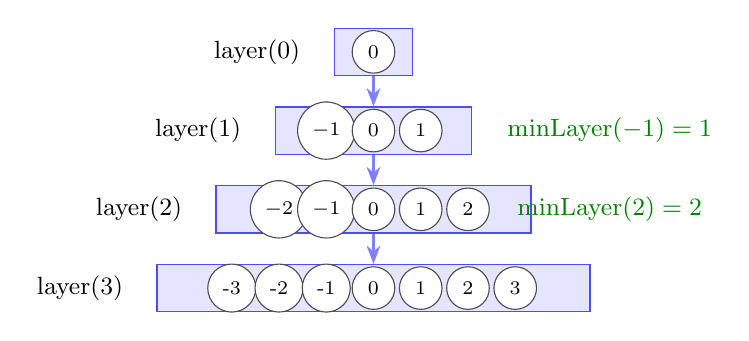
\begin{tikzpicture}[
    layer/.style={draw=blue!70, fill=blue!10, minimum height=0.6cm},
    elem/.style={circle, draw=black!70, fill=white, minimum size=0.4cm, font=\scriptsize}
]
% 層 0
\node[layer, minimum width=1cm] (l0) at (0, 3) {};
\node[left=0.3cm of l0, font=\small] {$\Layer(0)$};
\node[elem] at (0, 3) {0};

% 層 1
\node[layer, minimum width=2.5cm] (l1) at (0, 2) {};
\node[left=0.3cm of l1, font=\small] {$\Layer(1)$};
\node[elem] at (-0.6, 2) {$-1$};
\node[elem] at (0, 2) {0};
\node[elem] at (0.6, 2) {1};

% 層 2
\node[layer, minimum width=4cm] (l2) at (0, 1) {};
\node[left=0.3cm of l2, font=\small] {$\Layer(2)$};
\node[elem] at (-1.2, 1) {$-2$};
\node[elem] at (-0.6, 1) {$-1$};
\node[elem] at (0, 1) {0};
\node[elem] at (0.6, 1) {1};
\node[elem] at (1.2, 1) {2};

% 層 3
\node[layer, minimum width=5.5cm] (l3) at (0, 0) {};
\node[left=0.3cm of l3, font=\small] {$\Layer(3)$};
\foreach \x in {-3,-2,-1,0,1,2,3} {
    \node[elem] at (\x*0.6, 0) {\x};
}

% 矢印
\draw[-Stealth, blue!50, thick] (l0.south) -- (l1.north);
\draw[-Stealth, blue!50, thick] (l1.south) -- (l2.north);
\draw[-Stealth, blue!50, thick] (l2.south) -- (l3.north);

% minLayer の図示
\node[green!50!black, font=\small] at (3, 2) {$\minLayer(-1) = 1$};
\node[green!50!black, font=\small] at (3, 1) {$\minLayer(2) = 2$};
\end{tikzpicture}
\caption{整数絶対値塔：$\minLayer = |{\cdot}|$}
\label{fig:int-abs-tower}
\end{figure}

\begin{theorem}
整数絶対値塔はすべての公理を満たす。
\end{theorem}

\begin{proof}
\textbf{被覆性}：$x \in \Layer(|x|)$。
\textbf{単調性}：$|k| \leq i \leq j \Rightarrow |k| \leq j$。
\textbf{最小性}：$x \in \Layer(n) \Leftrightarrow |x| \leq n$ なので $\minLayer(x) = |x|$。
\end{proof}

%-----------------------------------------------------------------------------
\subsection{codepthTower：順序双対}

\begin{example}[codepth 塔]
順序を反転した「上からの層」。
\begin{align*}
    \Layer(n) &= \{k \in \N \mid n \leq k\} \\
    \minLayer(x) &= x \quad (\text{通常順序での最大})
\end{align*}
\end{example}

\begin{remark}
通常の順序では $i \leq j \Rightarrow \Layer(j) \subseteq \Layer(i)$（反単調）。
双対順序 $\N^{\mathrm{op}}$ では単調となる。
\end{remark}

%=============================================================================
\section{反例（Counterexamples.lean）}
%=============================================================================

\subsection{rankNotUniqueTower：最小層の非一意性}

\begin{counterexample}[非一意 minLayer 塔]
積順序（非線形順序）を添字とする塔。
\begin{align*}
    X &= \N \\
    I &= \N \times \N \quad (\text{積順序}) \\
    \Layer(i, j) &= \{k \in \N \mid k \leq i \lor k \leq j\}
\end{align*}
\end{counterexample}

\begin{figure}[htbp]
\centering
\begin{tikzpicture}[
    node distance=1.5cm,
    layer/.style={draw=blue!70, fill=blue!10, rounded corners, minimum width=2.5cm, minimum height=0.8cm},
    incomp/.style={draw=red!70, thick, dashed}
]

% 添字格子
\node[font=\bfseries] at (0, 3.5) {添字空間 $\N \times \N$};

\draw[->] (-0.5, 0) -- (3.5, 0) node[right] {$i$};
\draw[->] (0, -0.5) -- (0, 3) node[above] {$j$};

\foreach \i in {0,1,2,3} {
    \foreach \j in {0,1,2} {
        \filldraw[gray!50] (\i, \j) circle (2pt);
    }
}

% (1,0) と (0,1) を強調
\filldraw[red!70] (1, 0) circle (4pt) node[below right, font=\small] {$(1,0)$};
\filldraw[red!70] (0, 1) circle (4pt) node[above left, font=\small] {$(0,1)$};

% 比較不能を示す
\draw[incomp] (1, 0) -- (0, 1) node[midway, above right, font=\small, red!70] {比較不能};

% 層の内容
\node[layer] (l10) at (6, 2) {$\Layer(1,0) = \{0, 1\}$};
\node[layer] (l01) at (6, 0.5) {$\Layer(0,1) = \{0, 1\}$};

\node[green!50!black, font=\small] at (6, 1.25) {$1 \in$ 両方に属する};

\end{tikzpicture}
\caption{非一意 minLayer 塔：$(1,0)$ と $(0,1)$ は比較不能}
\label{fig:rank-not-unique}
\end{figure}

\begin{theorem}
非一意 minLayer 塔は被覆性・単調性を満たすが、minLayer が一意に定まらない。
\end{theorem}

\begin{proof}
\textbf{被覆性}：$x \in \Layer(x, x)$（$x \leq x$ より）。

\textbf{単調性}：$(i_1, j_1) \leq (i_2, j_2)$（つまり $i_1 \leq i_2 \land j_1 \leq j_2$）のとき、
\[
    k \in \Layer(i_1, j_1) \Rightarrow k \leq i_1 \lor k \leq j_1 \Rightarrow k \leq i_2 \lor k \leq j_2
\]
なので $\Layer(i_1, j_1) \subseteq \Layer(i_2, j_2)$。

\textbf{minLayer 非一意}：$1 \in \Layer(1, 0)$ かつ $1 \in \Layer(0, 1)$ だが、
\[
    (1, 0) \not\leq (0, 1) \quad \text{かつ} \quad (0, 1) \not\leq (1, 0)
\]
なので最小元が存在しない。
\end{proof}

\begin{remark}
この例は「$\minLayer$ が well-defined であるためには、添字集合 $I$ が線形順序（全順序）である必要がある」ことを示している。
\end{remark}

%=============================================================================
\section{公理の依存関係}
%=============================================================================

\begin{figure}[htbp]
\centering
\begin{tikzpicture}[
    axiom/.style={
        rectangle, rounded corners=5pt, draw=blue!70!black, 
        fill=blue!15, minimum width=2.8cm, minimum height=1cm,
        font=\bfseries, text=blue!70!black
    },
    example/.style={
        rectangle, rounded corners=3pt, draw=gray!70, 
        fill=gray!10, minimum width=2.5cm, minimum height=0.7cm,
        font=\small
    },
    ok/.style={-Stealth, thick, green!50!black},
    ng/.style={thick, red!60, dashed}
]

% 公理
\node[axiom] (cov) at (0, 2) {Covering};
\node[axiom] (mono) at (4, 2) {Monotone};
\node[axiom] (min) at (2, 0) {Minimality};

% 依存
\draw[ok] (cov) -- (min) node[midway, left, font=\scriptsize] {前提};
\draw[ok] (mono) -- (min) node[midway, right, font=\scriptsize] {前提};

% 独立
\draw[ng] (cov) -- (mono) node[midway, above, font=\scriptsize, red!60] {独立};

% 例の配置
\node[example, fill=green!20] at (-2, 0) {pointTower};
\node[example, fill=green!20] at (6, 0) {intAbsTower};
\node[example, fill=red!20] at (-2, -1.5) {singletonLayer};
\node[example, fill=orange!20] at (6, -1.5) {rankNotUnique};

\end{tikzpicture}
\caption{構造塔の公理と例の関係}
\label{fig:axiom-examples}
\end{figure}

%=============================================================================
\section{まとめ}
%=============================================================================

\begin{table}[htbp]
\centering
\caption{例の一覧と公理成立状況}
\label{tab:summary}
\small
\begin{tabular}{|l|c|c|c|l|}
\hline
\textbf{例} & \textbf{被覆} & \textbf{単調} & \textbf{最小} & \textbf{備考} \\
\hline
pointTower & $\checkmark$ & $\checkmark$ & $\checkmark$ & 最も自明 \\
singletonLayerTower & $\checkmark$ & $\times$ & — & 単調性失敗 \\
thresholdTower & $\checkmark$ & $\checkmark$ & $\checkmark$ & 閾値で飽和 \\
intAbsTower & $\checkmark$ & $\checkmark$ & $\checkmark$ & 標準例 \\
codepthTower & $\checkmark$ & 反単調 & $\checkmark$ & 双対順序 \\
rankNotUniqueTower & $\checkmark$ & $\checkmark$ & $\times$ & 非線形順序 \\
\hline
\end{tabular}
\end{table}

本稿で示した例は、構造塔理論における公理の必要性と添字順序の重要性を明確化する。
特に、rankNotUniqueTower は「$\minLayer$ の well-definedness には線形順序が必要」という
本質的な制約を示している。

%=============================================================================
% 参考文献
%=============================================================================

\begin{thebibliography}{9}

\bibitem{mathlib}
The mathlib Community.
\textit{Mathlib: The Math Library for Lean 4}.
\url{https://github.com/leanprover-community/mathlib4}

\bibitem{lean4}
Leonardo de Moura et al.
\textit{The Lean 4 Theorem Prover and Programming Language}.
CADE-28, 2021.

\end{thebibliography}

\end{document}
